\documentclass[12pt]{article}
%\documentstyle[12pt]{article}
\setlength{\oddsidemargin}{0in}
\setlength{\evensidemargin}{0in}
\setlength{\textwidth}{6.5in}
\setlength{\topmargin}{-.3in}
\setlength{\textheight}{9in}
\pagestyle{empty}

\usepackage[super]{nth}
\usepackage{amsmath}
\usepackage{csquotes}
\usepackage{physics}
\usepackage{graphicx}% Include figure files
\usepackage{dcolumn}% Align table columns on decimal point
\usepackage{bm}
\usepackage{subfig}

\begin{document}

\begin{center}
{\Large Doppler-Free Saturated Absorption Spectroscopy} \\
{\Large Lab Report} \\[.3in]
{\large Bj\"{o}rn Sumner and Benjamin Crane} \\
{13 Feb 2018}
\end{center}

\section*{Motivation and Context}

The atomic hyperfine structure arises from the interaction of the nuclear and electron magnetic moments.  This structure is responsible for many technological achievements, including the development of atomic clocks.  In fact, the SI second is defined by counting the number of transitions between two hyperfine states in the cesium 133 atom \cite{NISTsec}.  Additionally, the famous 21-cm line in astronomy is generated by a hyperfine transition in interstellar hydrogen\cite{21cmPred}.

The measurement of hyperfine splittings can be performed by using Doppler-Free Saturated Absorption Spectroscopy.  We will use this technique to measure the splittings of several hyperfine structures of Rubidium.

\section*{Physics and Predictions}

\subsection*{Atomic Spectra}
Rubidium is a hydrogen-like atom with a single $5s^1$ electron in its outer shell.  This electron gives rise to the two term states we will be interested in: $5^2\text{S}_{1/2}$ and $5^2\text{P}_{3/2}$.  There are two naturally occurring isotopes of Rubidium: $72\%$ abundant ${}^{85}\text{Rb}$ with spin number $I=5/2$ and $28\%$ abundant ${}^{87}\text{Rb}$ with $I = 3/2$.
The Hamiltonian describing the atom is given by
\begin{align}
	H &= \frac{p^2}{2m} - \frac{Z_{eff} e^2}{4 \pi \epsilon_0 r} + \zeta(r) \vec{L}\cdot \vec{S} \nonumber\\
	&\qquad + \alpha \vec{J}\cdot \vec{I} + \frac{\beta}{2I(2I-1)J(2J-1)}\left[3(\vec{I}\cdot \vec{J})^2 + \frac{3}{2}(\vec{I}\cdot \vec{J}) - I(I+1)J(J+1)\right] \label{eq:hamiltonian}
\end{align}


$\frac{p^2}{2m}$ contains the kinetic energy term and $- \frac{Z_{eff} e^2}{4 \pi \epsilon_0 r}$ the standard Coulomb attractive potential.  $\zeta(r) \vec{L}\cdot \vec{S}$ is the spin orbit coupling term, which gives rise to the broad term states such as $5^2\text{S}_{1/2}$ and $5^2\text{P}_{3/2}$.  The transition between these states is $780\,\text{nm}$.  The final two terms result from the hyperfine interaction.  The former term is the hyperfine interaction between the magnetic dipole of the nucleus and electron, while the latter comes from the nuclear electric quadrupole.  These two terms will produce the hyperfine states we will explore in this lab, and we label these states by their quantum number $F$, the magnitude of the total angular momentum $\vec{F} = \vec{J} + \vec{I}$.  The possible quantum numbers vary from $\rvert J-I\rvert$ to $J+I$.  These energy levels are shown in figure \ref{fig:RbEnergy}.  In this lab, we will look at ${}^{85}\text{Rb}$ transitions from $5^2\text{S}_{1/2}\,\text{F}=3$ to $5^2\text{P}_{3/2}\, \text{F'}=1,2,3,4$ and ${}^{87}\text{Rb}$ transitions from $5^2\text{S}_{1/2}\,\text{F}=2$ to $5^2\text{P}_{3/2}\, \text{F'}=0,1,2,3$.

\begin{figure}%
	\centering
	\subfloat[${}^{85}\text{Rb}$\cite{steck85Rb}]{{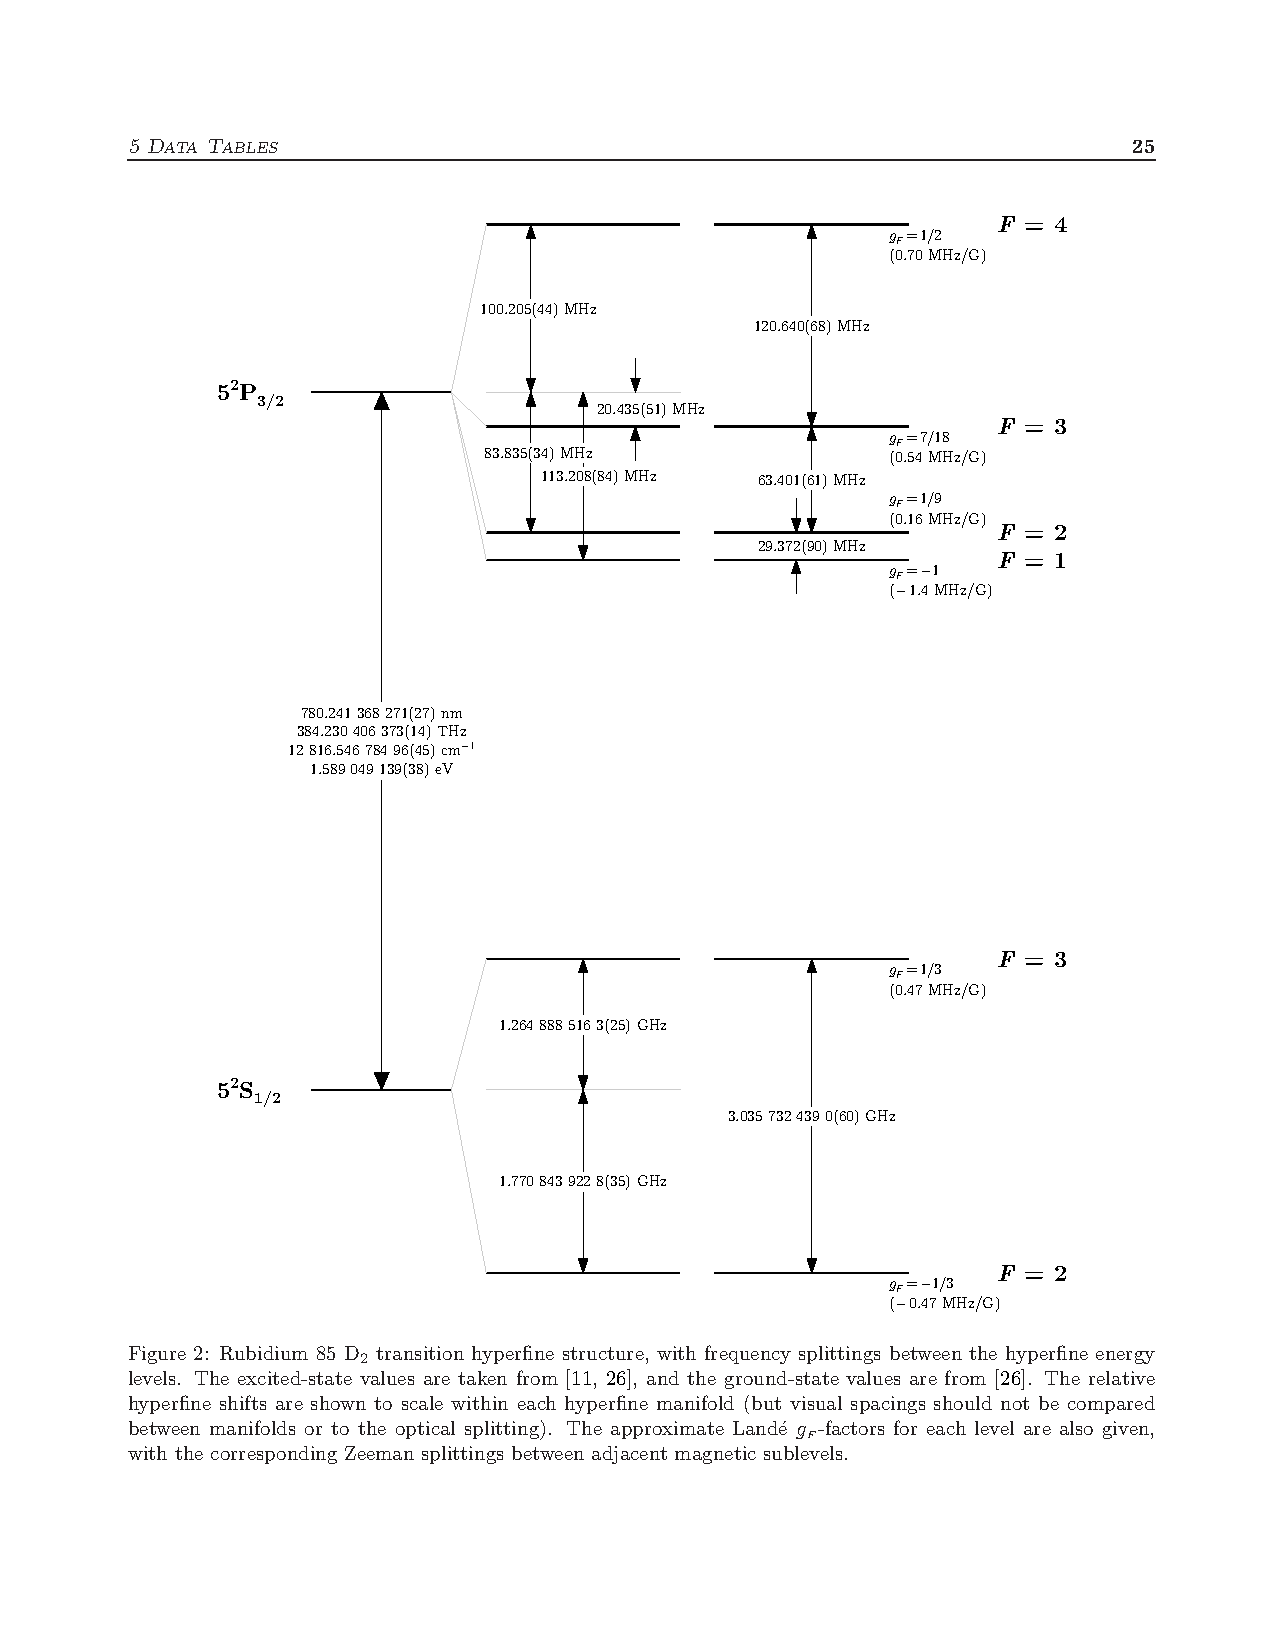
\includegraphics[width=8cm]{85D2.pdf} }}%
	\,
	\subfloat[${}^{87}\text{Rb}$\cite{steck87Rb}]{{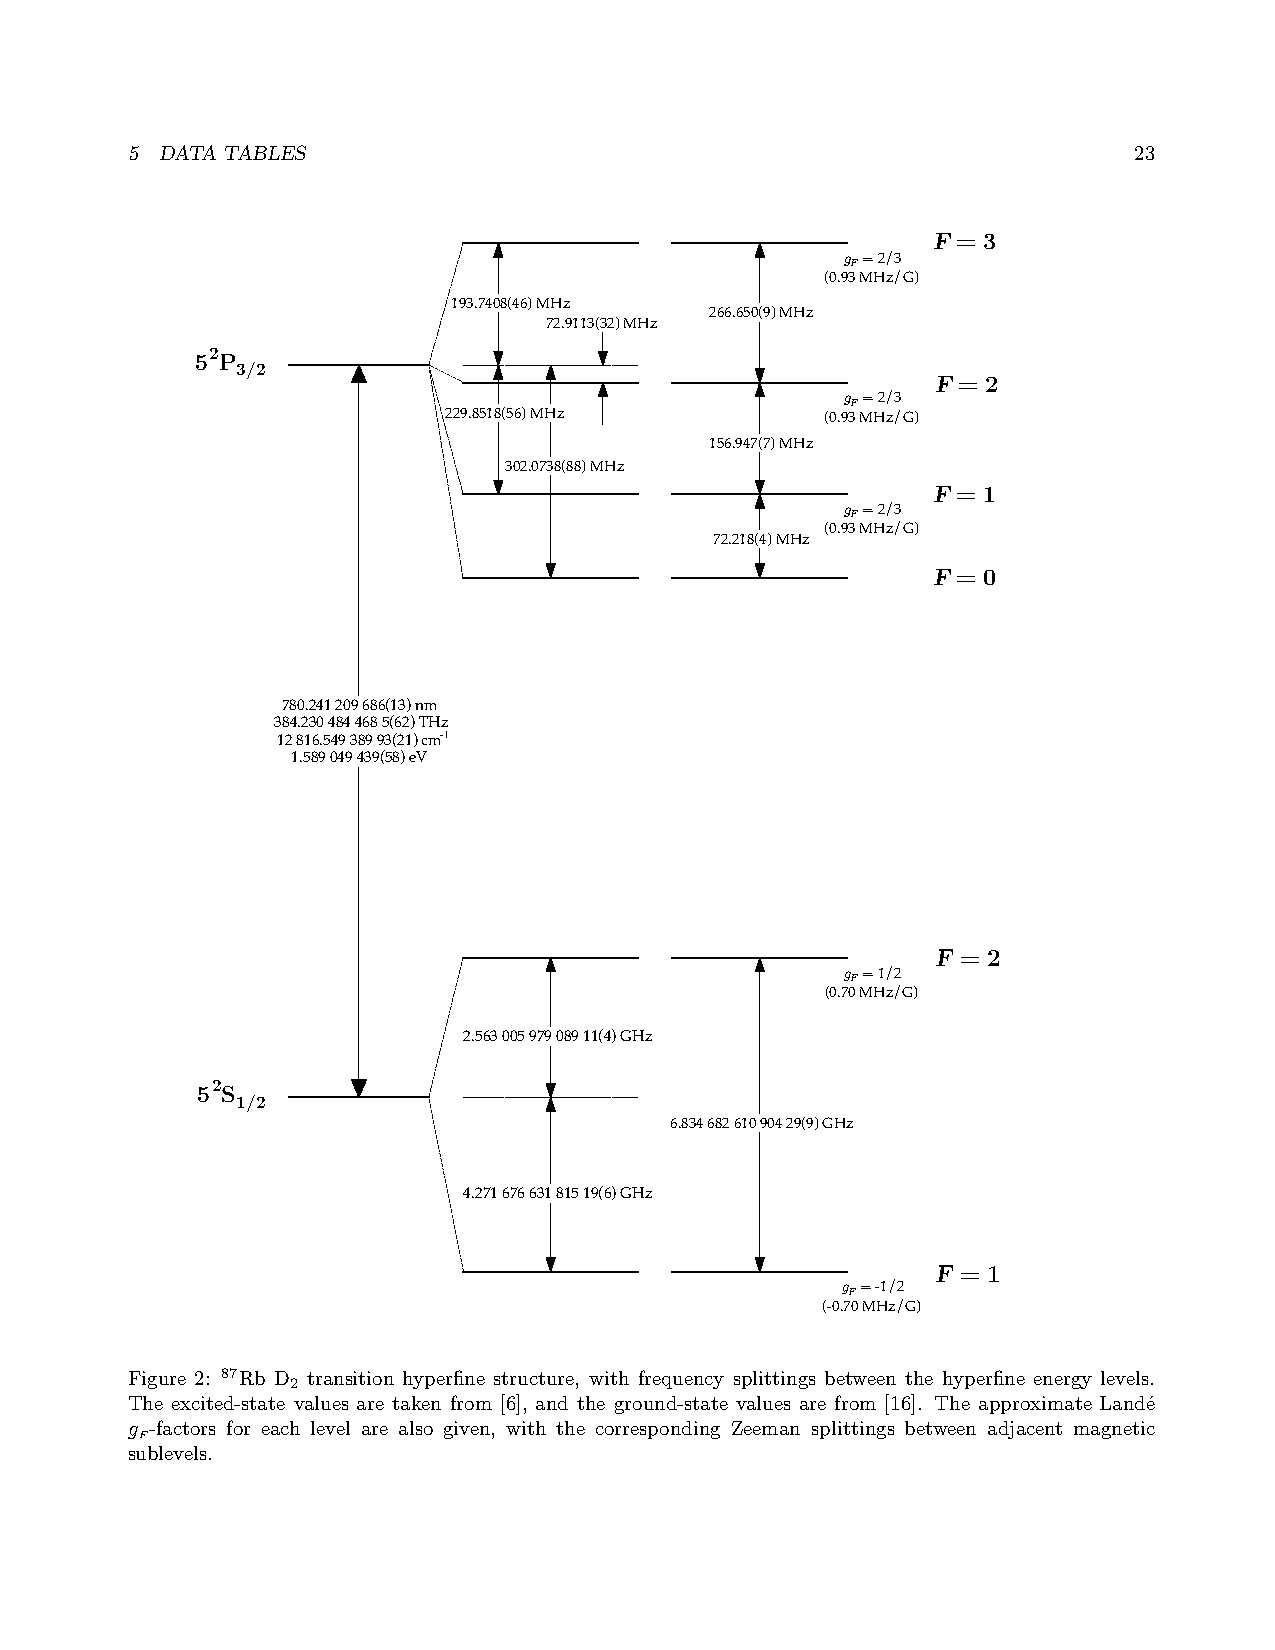
\includegraphics[width=8cm]{87D2.pdf} }}%
	\caption{Rubidium Energy Levels}%
	\label{fig:RbEnergy}%
\end{figure}

By using the Hamiltonian of equation \ref{eq:hamiltonian} in we can obtain the energies of the various hyperfine levels, and by dividing by Planck's constant, we can obtain an expression for the frequency associated with each level, indexed by quantum numbers $J$ and $F$:
\begin{align*}
	\nu_{J,F} &= \nu_J + A\frac{C}{2} + B \frac{\frac{3}{4}C(C+1) - I(I+1)J(J+1)}{2I(2I-1)J(2J-1)}
\end{align*}

where
$$C = F(F+1) - J(J+1) - I(I+1)$$

By taking the differences between these frequencies, we can obtain a prediction for the splittings between various hyperfine levels, which can then be used to predict the crossover levels.

\subsubsection*{${}^{85}\text{Rb}\,5^2\text{P}_{3/2}\,\text{Frequencies}$}

\paragraph{$F' = 4\, J = \frac{3}{2}\, I = \frac{5}{2}$}
\begin{align*}
C &= \frac{15}{2}\qquad
&\nu_{\frac{3}{2},4} = \nu_J + A \frac{15}{4} + B\frac{1}{4}= \nu_J +  \frac{75A+5B}{20}
\end{align*}

\paragraph{$F' = 3\, J = \frac{3}{2}\, I = \frac{5}{2}$}
\begin{align*}
	C &= -\frac{1}{2}\qquad
	&\nu_{\frac{3}{2},3} = \nu_J - A \frac{1}{4} - B\frac{11}{20}= \nu_J - \frac{5A+11B}{20}
\end{align*}

\paragraph{$F' = 2\, J = \frac{3}{2}\, I = \frac{5}{2}$}
\begin{align*}
	C &= -\frac{13}{2}\qquad
	&\nu_{\frac{3}{2},3} = \nu_J - A \frac{13}{4} - B\frac{1}{10} = \nu_J - \frac{65A+2B}{20}
\end{align*}

We thus predict the following splittings:
\paragraph{$F' = 2 \rightarrow 3$}

\subsection*{Doppler Broadening}

The spectra given in the previous section are obtained from a description of nature in the atom's frame of reference with no external effects.  However, real Rubidium atoms are subject to thermal motion, and as such these spectral lines will undergo broadening owing to the motion of the atoms relative to the laser.  Atoms moving toward the laser will `see' radiation blueshifted, and so absorption will only occur if the incoming photons are of a lower frequency than predicted by the spectra in figure \ref{fig:RbEnergy}.  Similarly, atoms moving away from the laser will absorb photons of higher frequency.  Because the velocity of these atoms follows the Maxwell distribution, it can be expected that the spectral lines will similarly follow such a distribution.  It can be shown that the half width of these distributions is given by 
\begin{align}
	\Delta \nu_{1/2} &= 2\frac{\nu_0}{c}\sqrt{\frac{2kT}{M}\ln(2)}
\end{align}

where $\nu_0$ is the rest frame atomic resonance, $M$ is the mass of the atom and $T$ is the temperature of the sample.

We can use this to predict the expected half width of the D2 lines.  Using figures from Steck\cite{steck85Rb}\cite{steck87Rb},

\subsubsection*{${}^{85}\text{Rb}\,\text{D}_2$}

\begin{align}
	\Delta \nu_{1/2} &= \frac{2}{\lambda_0}\sqrt{\frac{2kT}{M_{85}}\ln(2)}\nonumber\\
	&= \frac{2}{780.241\,\text{nm}}\sqrt{\frac{2\left(1.381\times10^{-23}\,\frac{\text{J}}{\text{K}}\right)\left(293\,\text{K}\right)}{1.410\times10^{-25}\,\text{kg}}\ln(2)}\nonumber\\
	&\approx 511 \text{MHz} \label{pred:85D2}
\end{align}

\subsubsection*{${}^{87}\text{Rb}\,\text{D}_2$}

\begin{align}
\Delta \nu_{1/2} &= \frac{2}{\lambda_0}\sqrt{\frac{2kT}{M_{87}}\ln(2)}\nonumber\\
&= \frac{2}{780.241\,\text{nm}}\sqrt{\frac{2\left(1.381\times10^{-23}\,\frac{\text{J}}{\text{K}}\right)\left(293\,\text{K}\right)}{1.443\times10^{-25}\,\text{kg}}\ln(2)}\nonumber\\
&\approx 505 \text{MHz}\label{pred:87D2}
\end{align}

These broadened spectra mask the hyperfine structure of the atoms, and so we must use Doppler-Free Saturated Absorption Spectroscopy to tease out these individual spectra.



\section*{Experiment and Data}

\subsection*{Experimental Setup}
We designed the experimental setup on the optical table to accommodate both portions of the lab in tandem, the Doppler-Free Saturated Absorption Spectroscopy and the Michelson Interferometer. The tedious process of finding and aligning the 780 nm external cavity diode laser took a long while. Using the Infrared-Viewing camera and the handheld cardviewer allowed us to trace the paths of Laser beam. The Laser beam was directed through a cube beam-splitter with the straight path continuing towards the Michelson Interferometer setup, and the perpendicular spit path towards a thick beam splitter. The thickness of the beam splitter allows for a precisely spaced set of parallel beams directly through the Rubidium vapor sample. These two weak beams are called the reference probe beam and the overlapping probe beam. The main portion of the laser continued straight through the thick beam splitter, becoming the start of the pump beam. The strong pump beam was angled with a mirror towards the opposite end of the table and was then angled with a separate mirror to align an overlap of the pump and the overlapping probe beam. These two beams are propagating in opposite directions. The overlapping probe beam continues through the rubidium vapor sample and is then directed with a mirror onto the photodetector. The reference probe beam is also reflected from a mirror through an optical attenuator and onto a separate photodetector. To achieve comparable power from the two probe beams we used a translation stage holding the variable attenuator to reduce the intensity of the reference beam. This was done visually with the aid of the oscilloscope  displaying the two channels of the photodetectors. 

The initial straight beam, passing through the cube-splitter, was incorporated into the Michelson Interferometer; this was accomplished by placing a thin microscope slide at ~45$^{\circ}$ to act as a 50-50 beam splitter. The longer reflected leg of the Michelson Interferometer was measured at a distance of 388.5 $\pm $0.5 mm, while the shorter straight leg was measured at a distance of 94.5 $\pm $0.5mm. The laser traveled down and back each leg of the Michelson Interferometer and recombined at the beamsplitter and travelled parallel to the photodetector and remained parallel all the way to the opposite wall. We experienced a lot of difficulty aligning the two beam to recombine at the third photodetector. After orienting the mirrors, beamsplitter and photodetector we noticed an odd feedback signal occurring on our oscilloscope. After discussing the feedback with Professor Jun Ye we were able to deduce the feedback was a result of setting the Michelson Interferometer and the doppler-free spectroscopy in tandem with each other. The reflections back through the beam splitter and back into the cube-splitter were resulting in feedback noise. To negate these effects we installed another variable optical attenuator, at an angle, between the cube splitter and microscope slide, to reduce the intensity and angle the reflection away. After its installation the signals cleared up and revealed 6 distinct peaks of the saturated absorption spectrum. Using the Math function of the oscilloscope we were able to subtract the doppler-broadened spectral lines with hyperfine structure (overlapping probe) from the Doppler-broadened spectral lines (reference probe) we were able to display just the specific peaks of the hyperfine structure. 

Toggling the Vortex Laser controls for the voltage and the wave-function generator's frequency and peak-to-peak voltage allowed for panning left and right and zooming in and out on specific portions, focusing on the hyperfine splitting of the 5$^2P_{3/2} $ state.  We decided to arrange the output from the Michelson Interferometer to be displayed along side the three other signals, allowing for a direct comparison. Channel one was displaying Doppler-broadened spectral lines with hyperfine structure, channel two was displaying the Doppler-broadened spectral lines, Channel three was the fringes of the Michelson interferometer, while channel four was the trigger signal from the wave-function generator. By incorporating all of the signals, onto the same oscilloscope we were able to directly overlay all of the information on comparable scales and then measure the fullwidth at half max  of the doppler broaden-lines of Rb$^{87} $ as well as the separation of the hyperfine lines for the F=2 to F' transition. We were then able to solve for the constants A and B of the 5$^2 P_{3/2}$.


\begin{figure}%
	\centering
	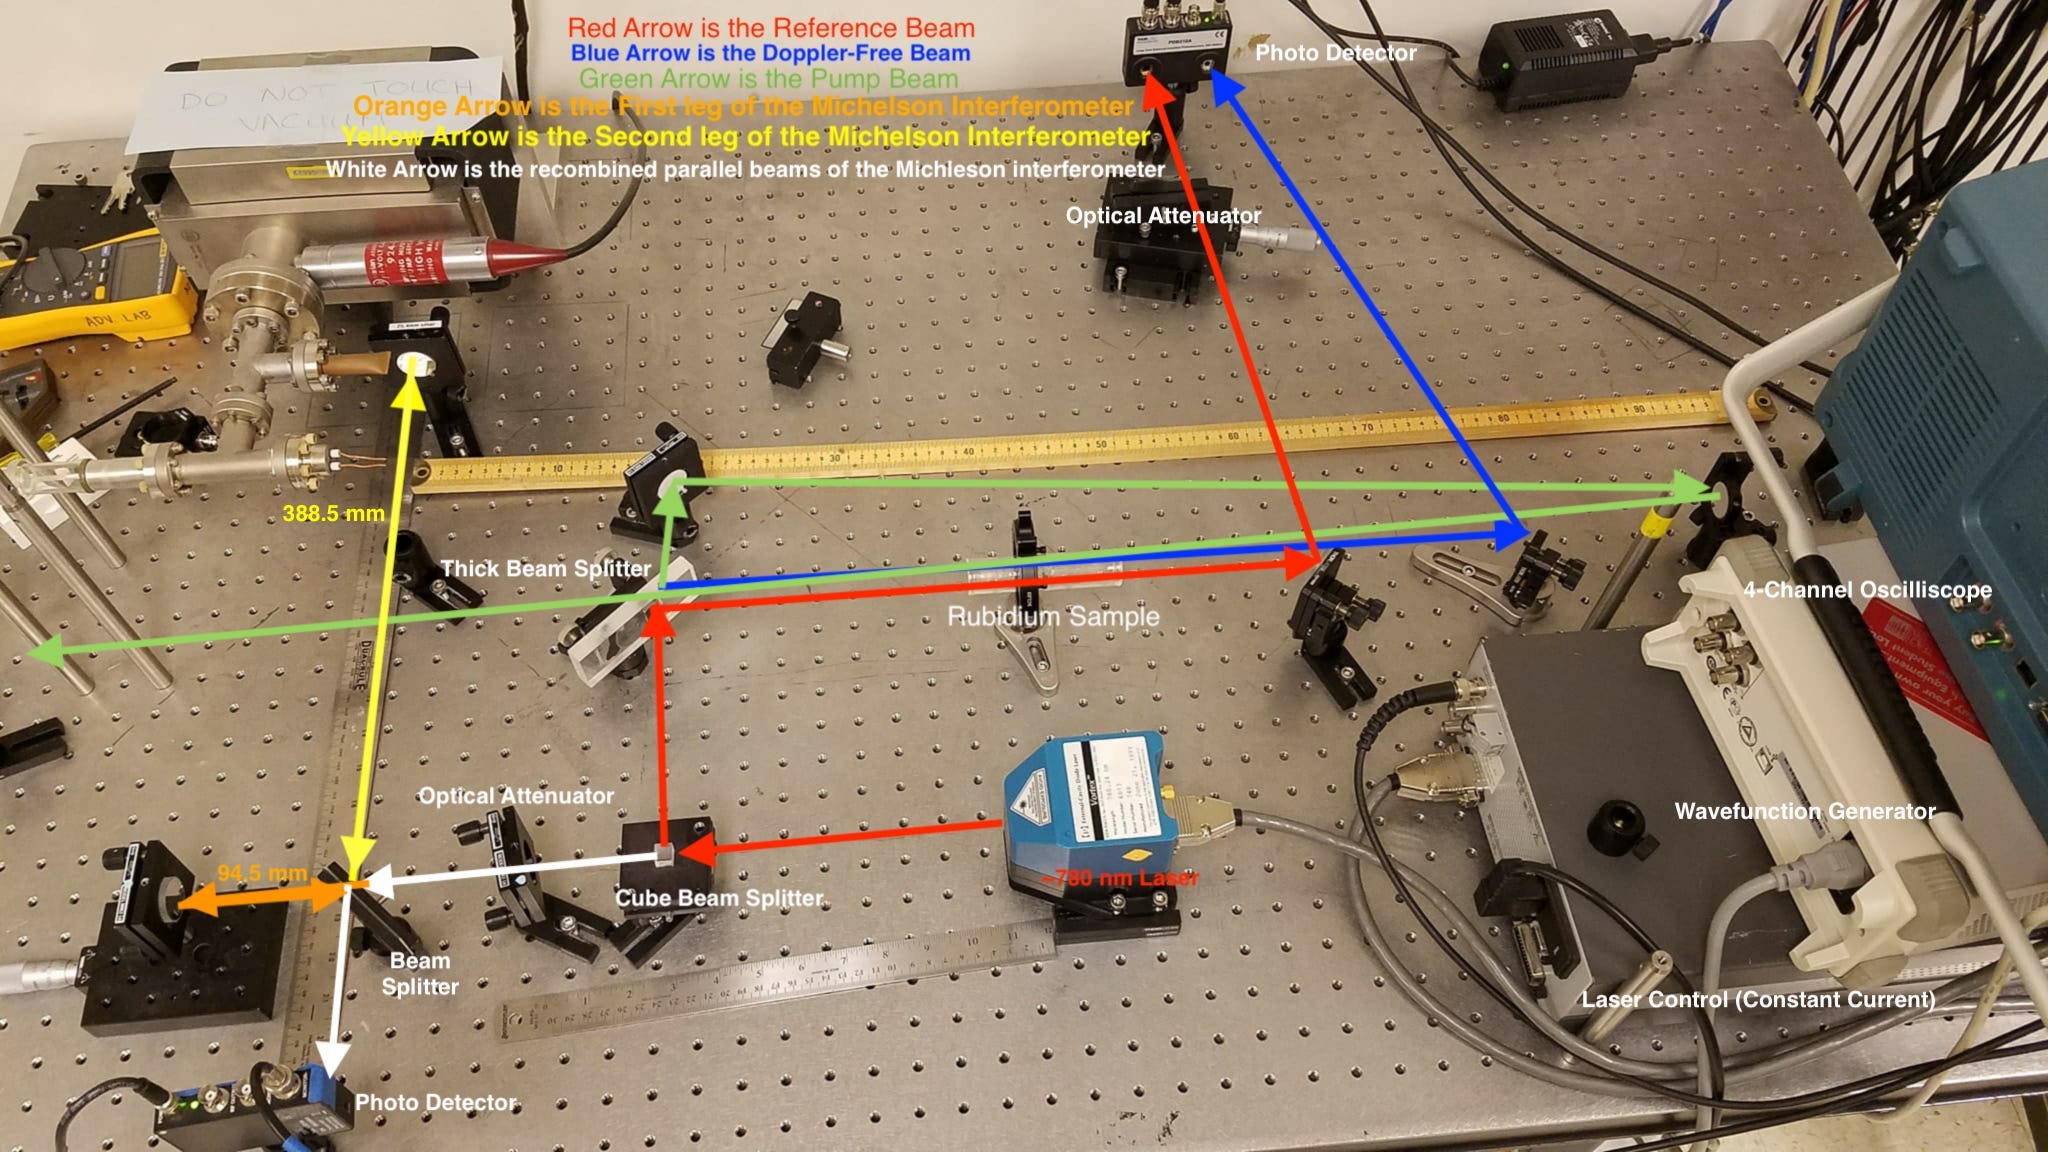
\includegraphics[width=\textwidth]{DFS_Layout.jpg}
	\caption{Experiment Layout}%
	\label{fig:Layout}%
\end{figure}

\subsection*{Results}

\subsection*{Error Analysis}

\section*{Conclusions}



\bibliographystyle{unsrt}
\bibliography{DFS_ref}

\end{document}
